\chapter{Laboratorio 1}
In questa esperienza di laboratorio si è realizzato e analizzato il seguente circuito:
\begin{figure}[h!]
	\centering
	\begin{minipage}{.4\textwidth}
	\scalebox{.9}{
		\begin{circuitikz}
			\draw (0,.5) node[ground]{};
			\draw (0,2) to[sV=$v_{in}$] (0,.5);
			\draw (0,2) to[R=$R_2$, -*] ++(3,0) ++(0.1,-.1) node[below]{$V^-$};
			\draw (3,2) to (4,2);
			\draw (3.7,2) node[op amp, anchor=-](oa){\texttt{TL071}};
			\draw (3.7,.5) node[ground]{} to[short, -*] (3.7,1);
			\draw (3,2) -- ++(0,1.3) coordinate(C) to[C=$C_1$] ++(3.08,0) (C-|oa.out) coordinate(Co) -- (oa.out) to [short, *-o] ++(1,0) node[above]{$v_{out}$};
			\draw (3,3.3) -- ++(0,1.3) to[R=$R_1$] ++(3,0) -| (Co);
			\draw[thick] (-.7,-.5) rectangle (7.65,5.5);
		\end{circuitikz}
	}
	\end{minipage}
	\qquad\qquad
	\begin{minipage}{.463\textwidth}
		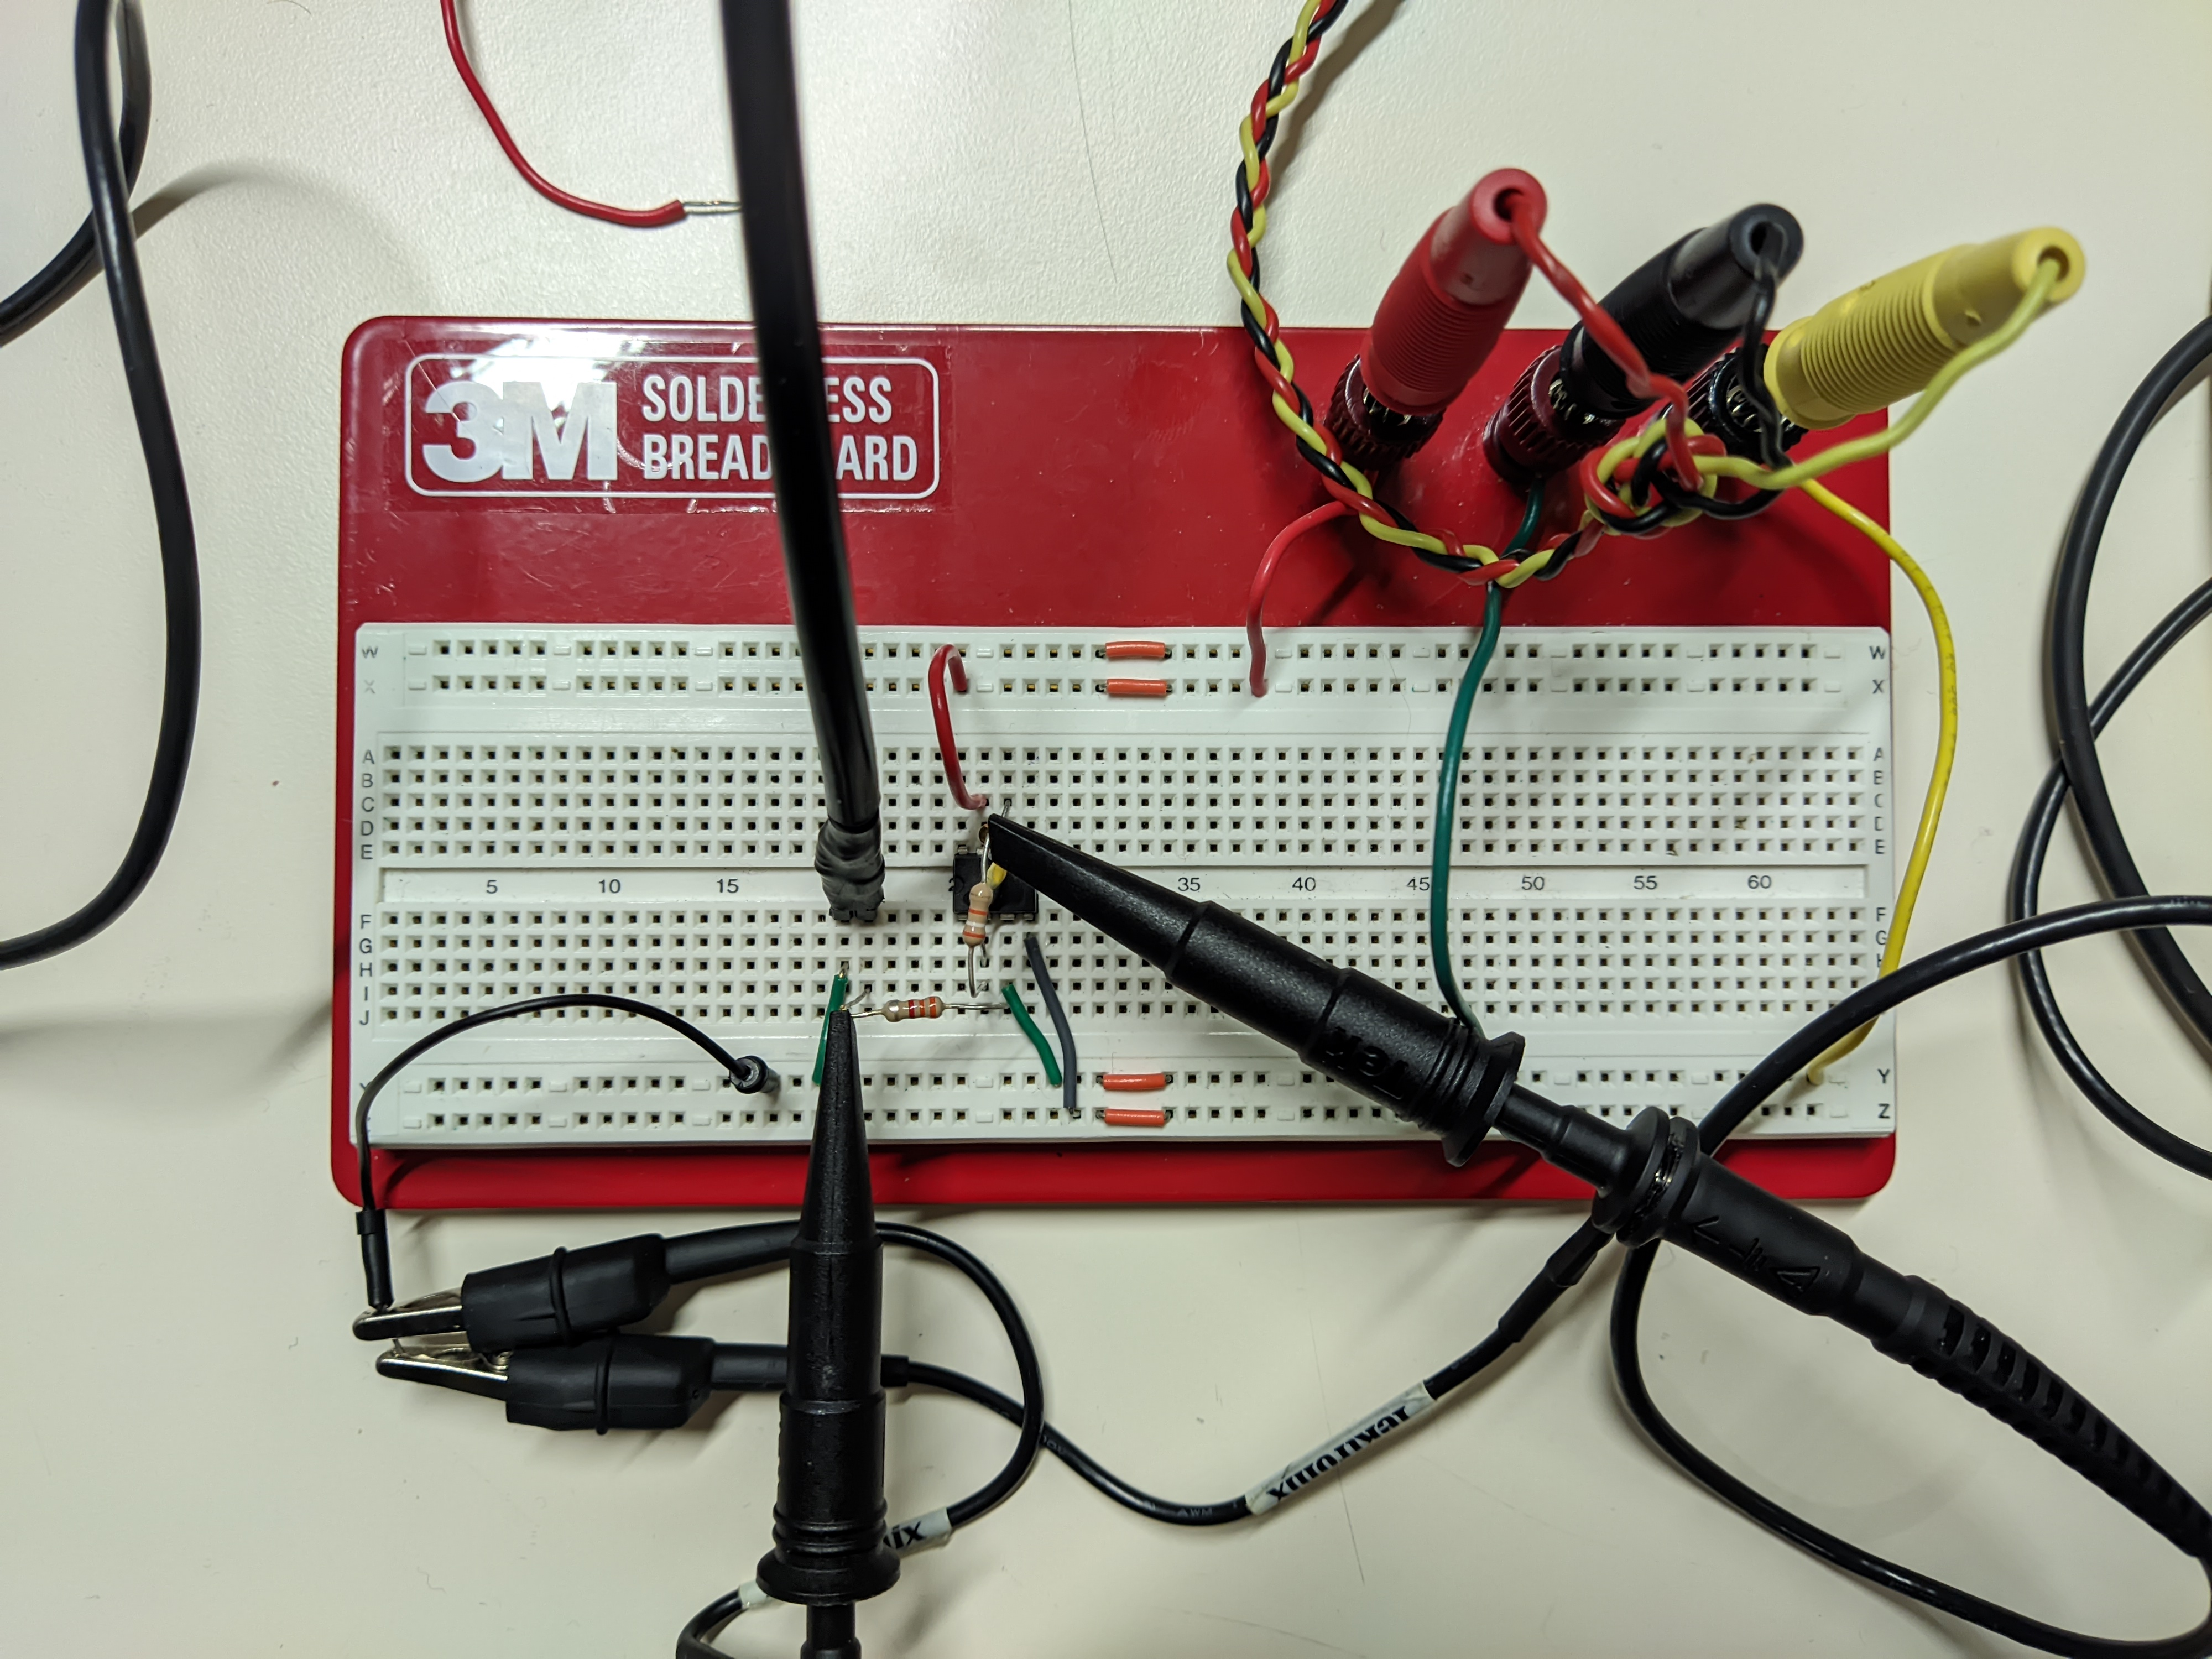
\includegraphics[width=\linewidth]{./ImageFiles/Laboratorio 1/CIRC.jpg}
	\end{minipage}
	\caption{Schema circuitale e foto circuito}
	\label{fig:circuito}
\end{figure}

Il circuito realizza un filtro passa basso attivo del primo ordine, utilizzando un amplificatore operazionale retroazionato negativamente. Infatti, è possibile ricavare la funzione di trasferimento del circuito tramite un bilancio delle correnti al nodo V\super{-}. Si consideri v\sub{in} come un generatore ideale di tensione applicato in ingresso al circuito. Indicando con Z\sub{1} l'impedenza equivalente del parallelo tra R\sub{1} e C\sub{1} e con Z\sub{2} l'impedenza della resistenza R\sub{2}, si può ottenere la funzione di trasferimento del circuito:
\begin{equation}
	v_{out}=-\frac{Z_1}{Z_2}v_{in}=-\frac{R_1}{R_2}\frac{1}{1+j w R_1 C_1} v_{in},
\end{equation}
da cui si ricava
\begin{equation}
	T=\frac{v_{out}}{v_{in}}=-\frac{R_1}{R_2}\frac{1}{1+j w R_1 C_1}.
\end{equation}
Questa funzione di trasferimento corrisponde a un filtro passa basso. È possibile calcolare il valore del modulo e della fase in funzione di $\omega$ tramite le seguenti espressioni:
\begin{equation}
	\begin{split}
		|T|&=\frac{R_1}{R_2}\frac{1}{\sqrt{1+(wR_1C_1)^2}} \\
		\angle T&=\SI{180}{\degree}-arctan(\omega R_1 C_1).
	\end{split}
\end{equation}
Per comprendere l'andamento del modulo e della fase in funzione della frequenza del segnale applicato in ingresso, è necessario analizzare i termini dipendenti da $\omega$ nelle due equazioni. Nell'espressione del modulo della funzione di trasferimento, il termine 
\begin{equation}
	\sqrt{1+(wR_1C_1)^2} \to
	\begin{cases}
		1 \; per \; \omega \to 0 \\
		\infty \; per \; \omega \to \infty
	\end{cases}
,
\end{equation}
mentre nell'espressione della fase, il termine
\begin{equation}
	arctan(\omega R_1 C_1) \to
	\begin{cases}
		0 \; per \; \omega \to 0 \\
		90^\circ \; per \; \omega \to \infty
	\end{cases}
	.
\end{equation}


Il modulo quindi tende a $\frac{R_1}{R_2}$ per segnali in ingresso a bassa frequenza, mentre tende a zero per segnali in ingresso ad alta frequenza, mentre la fase è pari a circa \SI{180}{\degree} per segnali a bassa frequenza, e tende a \SI{90}{\degree} per segnali ad alta frequenza.\todo{da sistemare questa parte}
Il comportamento del circuito è quindi quello di un filtro passa basso invertente del primo ordine, con frequenza di taglio pari a $f=\frac{1}{2\pi R_1C_1}$.

I valori dei componenti passivi sono stati scelti per soddisfare i requisiti di prestazioni del filtro. In particolare, veniva richiesto un guadagno di un fattore 10 con frequenza di taglio pari a \SI{10}{\kilo\hertz}. I valori nominali ed effettivi dei componenti passivi sono riportati in tabella \ref{tab:valori_componenti}.
\def\arraystretch{1.3}
\begin{table}[h]
	\centering
	\begin{tabular}{|c|c|c|}
		\hline
		Componente	& Valore Nominale & Valore Effettivo \\ \hline
		R1          & 3.3K\si{\ohm} &                   \\ \hline
		R2          & 38K\si{\ohm} &                   \\ \hline
		C1          & 390p\si{\farad} &                   \\ \hline
		
	\end{tabular}
	\caption{Valori nominali ed effettivi dei componenti passivi del circuito.}
	\label{tab:valori_componenti}
\end{table}

Attraverso un generatore di funzioni è stato applicato in ingresso al circuito una sinusoide con ampiezza picco-picco pari a \SI{500}{\milli\volt} e frequenza compresa tra \SI{100}{\hertz} e \SI{10}{\mega\hertz}. Tramite l'oscilloscopio sono state ottenute le misure di ampiezza picco-picco del segnale in uscita al circuito e la differenza di fase tra il segnale in ingresso e quello in uscita. Grazie a questi valori sono stati ricostruiti i diagrammi di Bode di modulo e fase del circuito, riportati in figura \ref{fig:diagrammi_di_Bode}.

\begin{figure}[h!]
	\centering
	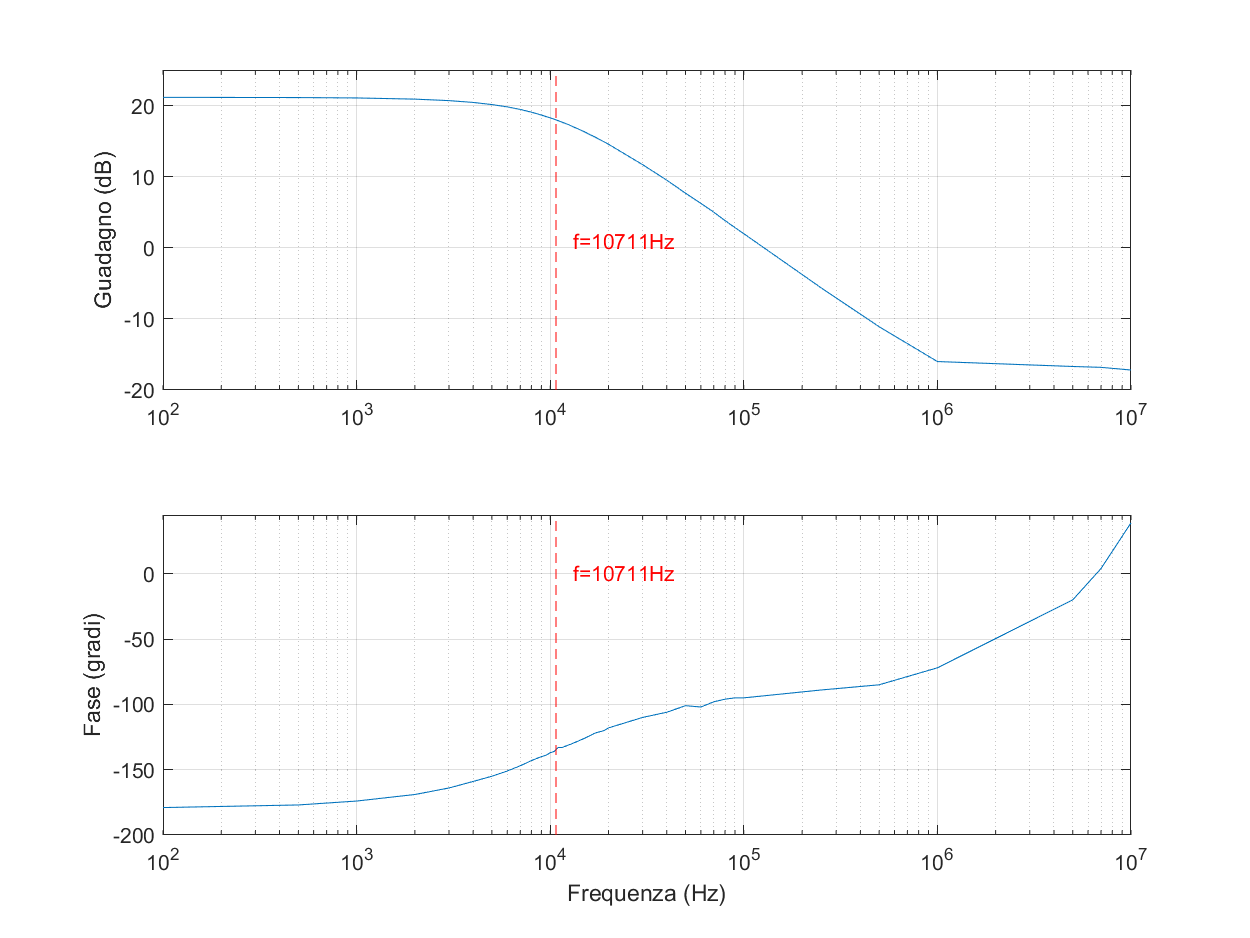
\includegraphics[width=\linewidth]{./ImageFiles/Laboratorio 1/Diagrammi di Bode.png}
	\caption{Diagrammi di Bode del filtro passa basso attivo del primo ordine.}
	\label{fig:diagrammi_di_Bode}
\end{figure}

Dai diagrammi di Bode della funzione di trasferimento si può osservare il comportamento del filtro passa basso:
\begin{itemize}
	\item osservando il diagramma di Bode del modulo si può notare che fino alla frequenza di taglio del circuito, che è pari a \SI{10711}{\hertz}, il segnale in ingresso viene amplificato di circa \SI{20}{\decibel}, mentre per valori superiori alla frequenza di taglio viene attenuato con una pendenza pari a \SI{20}{\decibel}/dec;
	\item osservando il diagramma di Bode della fase si può notare che, in corrispondenza della frequenza di taglio, la fase è diminuita di circa 45$^{\circ}$rispetto alle frequenza più basse, mentre una decade dopo la frequenza di taglio raggiunge i -90$^{\circ}$.
\end{itemize}

Tuttavia, per frequenze superiori ad \SI{1}{\mega\hertz}, il comportamento del circuito non è più quello descritto dalla formula \ref{1.3}\todo{link alla equazione}: infatti, a tali frequenze subentrano dei limiti dell'amplificatore operazionale per cui il sistema non è più retroazionato. \todo{Verificare questa informazione, lo ha detto Gaioni ma non è stato preciso}



\todo{inserire prove di saturazione}
\todo{inserire prove di offset}
